\documentclass[11pt]{extarticle}
\usepackage[utf8]{inputenc}
\usepackage{amsmath}
\usepackage{graphicx}
\usepackage[margin=1in]{geometry}

\title{\textbf{`` Grab 'em by the Fallacy "\\Stance Detection to Identify Fake News \\
  \large CS585, UMass Amherst, Fall 2017}}
\author{
$\textbf{Ajinkya Zadbuke}\quad\textbf{Arhum Savera}$\\
$\texttt{azadbuke@cs.umass.edu}\quad\texttt{asavera@umass.edu}$}
\date{}
\begin{document}

\maketitle

\section{Outline}
With the constant deluge of information available through multiple sources, it is more important than ever to be able to distinguish between factual and fabricated reports. Fake news, defined by the New York Times as 'a made up story with an intention to deceive' has been widely cited as a contributor to the outcome of the 2016 US elections. The Fake News Challenge was organized as a response to this controversy [1]. It is a public competition with the goal of using AI to automatically identify fake news. In this project, we aim to implement a solution for detecting stance in news articles, comparing multiple approaches and models. Our primary interest is in applying deep learning architectures such as Feed-forward Neural Networks, RNNs and LSTMs for this problem.

\section{Literature Review}

Paper [2] experiments with Conditional LSTM encoding in context of a tweet-to-target model, with a slightly different labelling scheme. It involves encoding the target as a fixed-length vector, and then the tweet with state intialized as the target’s repesentation. The final output of the tweet LSTM is used to predict the stance label for the pair.\\


Paper [3] tackles the same fake news dataset that we are using, implementing a Concatenated Multi-Layer Perceptron model, with Bag of Words representations and GLoVE Embeddings. They have also tried RNN and LSTM models, with the MLP performing better than the others.\\

Paper [4] also tackles the problem of fake news detection but uses a combination of linguistic cue approaches (with machine learning) and network analysis approaches. They experimented with BoW, Probabilistic Context-Free Grammars and SVMs while taking Social Network behavior and linked data properties into account.\\

Paper [5] introduces the Emergent data set that we will be using in our project. The authors also present their approach for stance detection where a regularized logistic regression classifier is used and features are extracted from the headline and the associated claim. The performance of the model is comparable to the state of the art stance detection. This team summarized each article into a headline and used a logistic regression model with features representing the article and claim to classify the combination of article and claim as either “for,” “against,” or “observing,” with a final accuracy level of 73%. \\

Paper [6] reported that using conditional encoding of LSTM models coupled with neural attention mechanisms have impressive results in detecting textual entailment. This task is conceptually similar to stance detection. Two sentences are input and the task is to determine if the sentences are unrelated, contradict each other, or if the second sentence is a logical consequence of the first sentence.\\
Before stance detection, closely related research, Natural language inference, focused on analyzing the relationship between two short sentences. Paper [7] explores a range of approaches to the problem of natural language inference beginning with methods which are robust but approximate, and proceeding to progressively more precise approaches.and attempts to infer if a given hypothesis can be inferred from a given premise.\\


Paper [8] focused on stance detection in tweets and tried to analyze the relationship between tweets and their views on specific topics. Given a tweet and a target entity, they determine whether the tweeter is in favor of the given target, against the given target, or whether neither inference is likely. They used SVM-ngrams and other simple linear classifiers using BOW for stance detection. \\

Paper [9] also tackles the problem of natural language inference, the authors introduced a new corpus of sentence pairs labeled for entailment, contradiction, and independence. They found that simple lexicalized models and neural network models perform considerably well.\\


\section{Datasets}
The dataset we will use is the one provided for the original FNC task [5]. This is a collection of articles, each consisting of a (headline, body, stance). The stance, which is our label, in this case, is one of \{unrelated, disagree, agree, discuss\}. The dataset has been created and annotated by accredited journalists, so we are not concerned with verifying quality of the data. We have 1648 headlines and 1669 article bodies, which have paired to create 49972 body-headline pairs. The data is inherently imbalanced as a result of the pairwise combinations, such that around 73\% of the examples are labeled as 'unrelated' with the rest distributed between 'discuss', 'agree' and 'disagree'. Considering this, the evaluation scheme we use is weighted (3:1) to prefer reward stance classification more than relatedness. The below figures show length of the article bodies and headlines in tokens.

\begin{center}
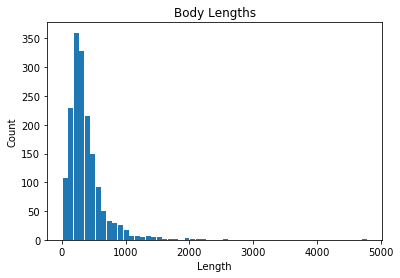
\includegraphics[width=8cm, height=6cm]{Dataset-body.png}
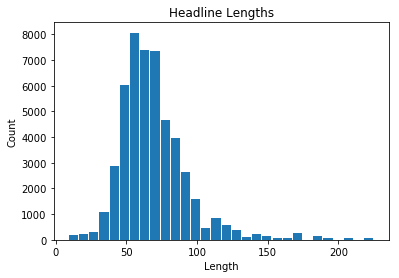
\includegraphics[width=8cm, height=6cm]{dataset-headlines.png}
\end{center}

\section{Evaluation}
Keeping with the spirit of the challenge, we will follow their evaluation guidelines. This involves handling the class imbalance by assigning a 25-75 weighting for the 'unrelated' and other classes, respectively. The baseline accuracy provided by the challenge can serve as a good benchmark to judge our models against (currently at 79.53\%).

\section{Scope and Approach}
The scope of the project is constrained by the following.
Claims made by recognized newsworthy sources are not considered fake news, as well as articles with humorous or sarcastic intent, as opposed to fabricated claims about newsworthy people, or by disreputable sources. 
The scope is also constrained by the data we use. Given the data we have, we focus on stance detection for the above, rather than explicitly modelling the fake news problem. Truth labelling is a challenging task even for humans, and other tasks have been determined to be feasible but decidedly non-trivial [5].
Our approach will involve implementing increasingly complex models, starting from a simple Logistic Regression classifier, and moving on to deep neural architectures such as Recurrent Neural Networks and Long-Short-Term Memory Networks. We aim to compare and contrast the performance of these models on a development set to tune our model hyperparameters (using k-fold cross-validation), and evaluate final accuracy on the test set. The test set itself consists of around 1000 samples, with the distribution of the classes unknown.


\section{Features}
\subsection{Word overlapping features}
The first feature is the jaccard similarity between the headline and the body of the article. After tokenizing the headlines and bodies, we calculate the Jaccard similarity for each headline and body pair.

\subsection{Refuting features}
We use a defined list of refuting words of length n with words such as 'fake','fraud','hoax','false' etc. and return a n dimensional binary vector for each headline with each dimension being 1 if the corresponding refuting word is present in the headline.

\subsection{Polarity features}
In this context, we define the polarity of a string to be 1 if it contains an odd number of refuting terms or 0 if it contains an even number of refuting terms. We use the same list of refuting words described above. We also define a polarity pair to be the polarity of a headline and body of an ariticle. We iterate over the articles and return a polarity pair for each article.

\subsection{N-Gram hits}
In our experiments, we use 2,3,4,5 and 6 grams. We compute the n-grams of the headline and then count how many times they appear in the body of the article. Additionally, we keep a separate count of how many common n-grams appear in the first 256 characters of the article body.

\subsection{Char-grams hits}
In our experiments, we use 2,4,8 and 16 character-grams. We compute the character-grams of the headline and then count how many times they appear in the body of the article. Additionally, we keep a separate count of how many common character-grams appear in the first 256 characters of the article body.

\subsection{Co-occurence count}
We tokenize the headline and body and count how many times a token in the headline occurs in the article body. We also keep a separate count for how many times common tokens appear in the first 256 characters of the article body.

\subsection{Co-occurence count without stop words}
We tokenize the headline and body, remove stop words, and count how many times a token in the headline occurs in the article body. We also keep a separate count for how many times common tokens appear in the first 256 characters of the article body.

\section{Results}
\begin{center}
 \begin{tabular}{||c c c c c c||} 
 \hline
  & Logistic Regression & Gradient Boosting & Random Forest  & BoW NN & Multilayer Perceptron \\  
 \hline\hline
 \hline fold 0 & 0.767 &  0.790 & 0.796 & 0.842 & 0.760    \\ [1ex] 
 \hline fold 1 & 0.769 &  0.793 & 0.797 & 0.790 & 0.769   \\ [1ex] 
 \hline fold 2 & 0.783 &  0.817 & 0.806 & 0.808 & 0.257   \\ [1ex] 
 \hline fold 3 & 0.785 &  0.810 & 0.822 & 0.830 & 0.742   \\ [1ex]  
 \hline fold 4 & 0.778 &  0.795 & 0.795 & 0.850 & 0.617   \\ [1ex] 
 \hline fold 5 & 0.748 &  0.764 & 0.779 & 0.798 & 0.424   \\ [1ex] 
 \hline fold 6 & 0.750 &  0.774 & 0.776 & 0.836 & 0.747   \\ [1ex] 
 \hline fold 7 & 0.769 &  0.806 & 0.794 & 0.808 & 0.567   \\ [1ex] 
 \hline fold 8 & 0.796 &  0.820 & 0.811 & 0.833 & 0.649   \\ [1ex] 
 \hline fold 9 & 0.758 &  0.787 & 0.786 & 0.827 & 0.786   \\ [1ex] 
 \hline Dev set score  & 76.138  & 79.976  & 68.686 & 84.25  & 77.92 \\ [1ex] 
 \hline Test set score &  72.711  & 75.200  & 74.097  & 75.35  & 74.47 \\ [1ex] 
 
 \hline
\end{tabular}
\end{center}
\section{References}

[1] Fake News Challenge - https://www.fakenewschallenge.org/

[2] Augenstein, I., Rocktaschel, T., Vlachos, A., Bontcheva, K., Stance Detection with Conditional Bidirectional Encoding, September 2016

[3] Fake News, Real Consequences: Recruiting Neural Networks for the Fight Against Fake News, January 2017

[4] Conroy, N., Rubin, V., Chen, Y. Automatic Deception Detection: Methods for Finding Fake News, November 2015

[5] Ferreira, W., and Vlachos, A., Emergent : A Novel Dataset for Stance Classification, June 2016

[6] Tim Rocktaschel, Edward Grefenstette, Karl Moritz Hermann, Tom Kocisky, and Phil Blunsom: Reasoning about Entailment with Neural Attention.Sep 2015.

[7] B. MacCartney, “Natural language inference.” 

[8] “Semeval-2016 task 6: Detecting Stance in Tweets” Saif M. Mohammad, Svetlana Kiritchenko,Parinaz Sobhani, Xiaodan Zhu, Colin Cherry

[9] Bowman, Samuel R., et al. "A large annotated corpus for learning natural language inference."  arXiv preprint arXiv:1508.05326,  2015.

\end{document}
